% ============================================================================
% Report 1 of 2: the VidFetch application (use, design, libraries, code).
% Independent of the data: compile with pdflatex/latexmk (twice).
% The results of the filmed tests are in informe_ensayos.tex.
% ============================================================================
\documentclass[11pt, a4paper]{article}
% ----------------------------------------------------------------------------
% Preamble: packages, language, units, colours and PGFPlots styles.
% ----------------------------------------------------------------------------
\usepackage[T1]{fontenc}
\usepackage[utf8]{inputenc}
\IfFileExists{lmodern.sty}{\usepackage{lmodern}}{}
\usepackage[a4paper, margin=2.3cm]{geometry}

% Spanish when available (TeX Live full / MiKTeX); otherwise English babel + Spanish names.
\IfFileExists{spanish.ldf}{%
  \usepackage[spanish, es-noshorthands, es-tabla]{babel}%
}{%
  \usepackage[english]{babel}%
  \addto\captionsenglish{%
    \renewcommand{\figurename}{Figura}\renewcommand{\tablename}{Tabla}%
    \renewcommand{\contentsname}{Índice}\renewcommand{\refname}{Referencias}%
  }%
}

\emergencystretch=2em   % avoid overfull lines with long \texttt file names
\usepackage{amsmath, amssymb}
\usepackage{graphicx}
\usepackage{float}
\usepackage{booktabs}
\usepackage{caption}
\captionsetup{font=small, labelfont=bf}
\usepackage{xcolor}

\usepackage{siunitx}
% Numbers arrive already rounded by generar_informe.py: no re-rounding (integers stay integers).
\sisetup{output-decimal-marker = {,}, group-separator = {\,}, group-minimum-digits = 5,
         round-mode = none, per-mode = symbol}
\DeclareSIUnit{\px}{px}

\usepackage{tikz}
\usetikzlibrary{positioning, fit, backgrounds, calc}
\usepackage{pgfplots}
\usepackage{pgfplotstable}
\pgfplotsset{compat=1.17}
\usepgfplotslibrary{fillbetween}
\pgfkeys{/pgf/number format/.cd, use comma, 1000 sep={\,}}

% Time-scale helpers: every frame <-> real-time equivalence in the text is computed from
% \CuadrosPorSegundo (config.tex), so changing that single value updates the whole report.
\newcommand{\FileFps}{29.97}   % playback rate of the DJI files [frames/s]
\newcommand{\CalcNum}[2][3]{\pgfmathsetmacro\calcres{#2}\num[round-mode=figures, round-precision=#1]{\calcres}}
\newcommand{\CalcQty}[3][2]{\pgfmathsetmacro\calcres{#2}\SI[round-mode=figures, round-precision=#1]{\calcres}{#3}}
\newcommand{\EnSeg}[1]{\CalcQty{#1/\CuadrosPorSegundo}{\second}}          % n frames -> real seconds
\newcommand{\Cuadros}[1]{\num{#1}~cuadros (\EnSeg{#1})}                    % "n cuadros (x s)"
\newcommand{\fr}{f_{\mathrm{r}}}
\newcommand{\fa}{f_{\mathrm{a}}}

\definecolor{azul}{RGB}{42,111,219}
\definecolor{rojo}{RGB}{211,51,51}
\definecolor{verde}{RGB}{34,160,60}
\definecolor{naranja}{RGB}{240,140,0}

% Cycle of 12 distinguishable colours for per-robot curves (repeats beyond 12 robots).
\pgfplotscreateplotcyclelist{robots}{
  {color=azul}, {color=rojo}, {color=verde}, {color=naranja}, {color=violet}, {color=teal},
  {color=brown}, {color=magenta}, {color=olive}, {color=cyan!70!black}, {color=gray}, {color=black}}

% Code listings (application report). Comments in the code are in English.
\usepackage{listings}
\definecolor{codefondo}{RGB}{246,247,249}
\definecolor{codecom}{RGB}{110,120,130}
\definecolor{codekw}{RGB}{42,111,219}
\definecolor{codestr}{RGB}{170,80,20}
\lstdefinestyle{py}{language=Python, basicstyle=\ttfamily\footnotesize, keywordstyle=\color{codekw}\bfseries,
  commentstyle=\color{codecom}\itshape, stringstyle=\color{codestr}, backgroundcolor=\color{codefondo},
  frame=single, rulecolor=\color{gray!40}, framesep=4pt, xleftmargin=6pt, xrightmargin=6pt,
  numbers=left, numberstyle=\tiny\color{gray}, numbersep=6pt, breaklines=true, showstringspaces=false,
  columns=fullflexible, keepspaces=true, upquote=true, tabsize=4, captionpos=b,
  literate={á}{{\'a}}1 {é}{{\'e}}1 {í}{{\'i}}1 {ó}{{\'o}}1 {ú}{{\'u}}1 {ñ}{{\~n}}1 {θ}{{$\theta$}}1 {ω}{{$\omega$}}1}
\lstset{style=py}
\renewcommand{\lstlistingname}{Código}
\renewcommand{\lstlistlistingname}{Índice de códigos}

\usepackage[hidelinks]{hyperref}
\usepackage{cleveref}
% Spanish reference names regardless of the babel language actually loaded.
\crefname{figure}{fig.}{figs.}\Crefname{figure}{Figura}{Figuras}
\crefname{table}{tabla}{tablas}\Crefname{table}{Tabla}{Tablas}
\crefname{section}{sección}{secciones}\Crefname{section}{Sección}{Secciones}
\crefname{subsection}{sección}{secciones}\Crefname{subsection}{Sección}{Secciones}
\crefname{lstlisting}{código}{códigos}\Crefname{lstlisting}{Código}{Códigos}\crefname{listing}{código}{códigos}\Crefname{listing}{Código}{Códigos}
\crefname{equation}{ec.}{ecs.}\Crefname{equation}{Ecuación}{Ecuaciones}
\creflabelformat{equation}{(#2#1#3)}

% ----------------------------------------------------------------------------
% Experiment-wide settings. Edit here; every section reads these macros.
% ----------------------------------------------------------------------------
% Titles of the two reports (informe_aplicacion.tex and informe_ensayos.tex).
\newcommand{\TituloAplicacion}{VidFetch: seguimiento de robots en video}
\newcommand{\SubtituloAplicacion}{Uso, funcionamiento y código de la aplicación}
\newcommand{\TituloEnsayos}{Robots autopropulsados confinados: resultados de los ensayos filmados}
\newcommand{\SubtituloEnsayos}{Posición, velocidad, rotación y atascos en tres ensayos con 22 robots}
\newcommand{\Autores}{Dylan Frigerio}
\newcommand{\Institucion}{ITBA}
\newcommand{\FechaInforme}{\today}

% Real robot diameter (same value as "Diámetro real" in the app; 33 mm, consistent with the image
% measured with the enclosure scale). It sets the wall-contact radius and the area fraction, not the scale.
\newcommand{\DiametroRobotCM}{3.3}

% Enclosure (recinto): inner and outer diameter of the wall ring. The px -> mm scale of every frame
% comes from the inner diameter (same values as "Diámetro interior/exterior" in the app).
\newcommand{\DiametroIntRecintoCM}{18.5}
\newcommand{\DiametroExtRecintoCM}{19.5}

% Time scale of the time-lapse videos: frames that correspond to 1 s of real time
% (same value as "Escala de tiempo" in the app; 3 by default).
\newcommand{\CuadrosPorSegundo}{3}


\title{\TituloAplicacion\\[2pt]\large \SubtituloAplicacion}
\author{\Autores \\ \small \Institucion}
\date{\FechaInforme}

\begin{document}
\maketitle

\begin{abstract}
\noindent VidFetch mide la posición, la velocidad, la orientación y la velocidad angular de $N$ robots
circulares filmados desde arriba. Detecta cada robot con un filtro adaptado a su forma (disco claro
rodeado de un anillo oscuro) y \texttt{trackpy.locate}, lo sigue con $N$ fijo mediante asignación
óptima y predicción, deriva la velocidad con un filtro de Savitzky--Golay y obtiene el giro comparando
firmas polares en el dominio de Fourier. Este informe explica para qué sirve, cómo está organizado,
qué bibliotecas usa y qué hace cada parte del código. Los resultados de los ensayos están en un
informe aparte.
\end{abstract}

\newpage
\tableofcontents
\newpage

% ============================================================================
% Application report: what it is, how it is organised, files it reads/writes.
% ============================================================================
\section{Qué es y para qué sirve}\label{sec:app}

VidFetch es una aplicación de escritorio en Python que mide, a partir de un video filmado desde
arriba, el movimiento de $N$ robots circulares dentro de una arena. Para cada robot y cada cuadro
entrega la posición del centro, el vector velocidad, la orientación acumulada $\theta$ y la
velocidad angular $\omega$, en unidades SI y en tiempo real aunque el video esté acelerado.

Usos previstos:
\begin{itemize}
  \item \textbf{Preparar el video}: recortar el tramo útil y el rectángulo de la arena, y guardar el
        recorte (archivos \texttt{VC\_}).
  \item \textbf{Probar la detección} sobre cuadros sueltos y ajustar parámetros a mano o con la
        calibración automática.
  \item \textbf{Seguir} $N$ robots fijos durante todo el ensayo, revisar los cuadros dudosos y
        corregir centros a mano.
  \item \textbf{Exportar} los datos (CSV), un resumen por robot, el video anotado y la sesión de
        análisis para retomarla sin volver a procesar.
  \item \textbf{Generar los informes} de ensayos a partir de los CSV (\cref{sec:procedimiento}).
\end{itemize}

\subsection{Requisitos y ejecución}

Requiere Python~3.10 o superior y las bibliotecas de \texttt{requirements.txt}
(\cref{sec:librerias}). Desde la carpeta \texttt{software/vidfetch} del repositorio:
\begin{verbatim}
pip install -r requirements.txt
python main.py
\end{verbatim}
Las tareas largas (análisis, exportaciones) corren en un hilo aparte, con barra de progreso y botón
de cancelar, de modo que la ventana no se congela.

\subsection{Organización del código}

El código separa la lógica de cálculo (\texttt{core/}, sin dependencias de la interfaz) de la
interfaz gráfica (\texttt{gui/}). Así, todo el cálculo puede usarse desde un script, y la interfaz
solo llama a funciones de \texttt{core/} (\cref{tab:archivos}).

\begin{table}[H]
  \centering
  \caption{Archivos del programa y su función (rutas relativas a \texttt{software/vidfetch}).}
  \label{tab:archivos}
  \small
  \begin{tabular}{@{}lrp{9.2cm}@{}}
    \toprule
    Archivo & Líneas & Función \\
    \midrule
    \texttt{main.py} & 18 & punto de entrada: crea la aplicación Qt y la ventana principal \\
    \texttt{core/models.py} & 47 & \texttt{Roi} (rectángulo) y \texttt{TrimRange} (tramo de cuadros) \\
    \texttt{core/video\_io.py} & 169 & lectura de video con acceso aleatorio, exportación de video recortado o anotado \\
    \texttt{core/processing.py} & 94 & operaciones de imagen encadenables (grises, brillo/contraste, desenfoque, umbral, Canny) \\
    \texttt{core/detection.py} & 182 & detección de robots: filtro de anillo, \texttt{trackpy.locate}, cobertura del anillo \\
    \texttt{core/calibration.py} & 230 & estimación automática del radio del robot y de todos los umbrales \\
    \texttt{core/analysis.py} & 116 & recorrido del video cuadro a cuadro y tabla de candidatos \\
    \texttt{core/tracking.py} & 708 & seguimiento con $N$ fijo, anclas manuales, huecos, sesión \texttt{.npz}, dibujo \\
    \texttt{core/rotation.py} & 139 & firmas polares y orientación acumulada $\theta$ \\
    \texttt{core/kinematics.py} & 250 & velocidad, $\omega$, escala SI y tablas de exportación \\
    \midrule
    \texttt{gui/main\_window.py} & 522 & ventana, menús, diálogos de archivo y tareas en segundo plano \\
    \texttt{gui/state.py} & 71 & estado compartido: video, tramo, rectángulo, escala de tiempo \\
    \texttt{gui/tabs.py} & 501 & pestañas \emph{Original}, \emph{Recortar} y \emph{Procesar} \\
    \texttt{gui/tracking\_tab.py} & 498 & pestaña \emph{Seguimiento} \\
    \texttt{gui/player.py}, \texttt{frame\_view.py} & 362 & reproductor y visor con zoom y edición del rectángulo \\
    \texttt{gui/export\_worker.py} & 35 & hilo de trabajo (\texttt{QThread}) para tareas largas \\
    \midrule
    \multicolumn{3}{@{}l}{\textit{En \texttt{software/analisis\_video/}:}} \\
    \texttt{generar\_informe.py} & 548 & sección de resultados de un ensayo a partir de su CSV \\
    \texttt{comparar\_ensayos.py} & 530 & comparación entre ensayos y contraste con el sensor de presión \\
    \bottomrule
  \end{tabular}
\end{table}

\subsection{La interfaz}

La ventana tiene cuatro pestañas que comparten el mismo video, tramo y rectángulo, guardados en
un único objeto de estado (\texttt{gui/state.py}): lo que se define en una se refleja en las demás.
\begin{enumerate}
  \item \textbf{Original}: reproduce el video y fija la escala de tiempo (\cref{sec:escala}). La
        etiqueta del reproductor muestra el cuadro y el tiempo real.
  \item \textbf{Recortar}: tramo temporal (cuadro de inicio y fin) y rectángulo de análisis, que se
        dibuja o se mueve sobre la imagen; permite forzar un cuadrado de lado fijo y guardar el recorte.
  \item \textbf{Procesar}: aplica operaciones de imagen y prueba la detección cuadro a cuadro
        (parámetros, botón \emph{Calibrar tamaño automáticamente}). Exporta posiciones sueltas o
        vinculadas con \texttt{trackpy.link} y el video procesado.
  \item \textbf{Seguimiento}: análisis completo con $N$ fijo, lista de cuadros con problemas,
        corrección manual del centro, parámetros de cinemática (ventana de suavizado, diámetro real,
        corrección de video espejado),
        superposición de velocidad y orientación, y exportaciones.
\end{enumerate}

\subsection{Archivos que lee y escribe}

\begin{table}[H]
  \centering
  \caption{Formatos de archivo.}
  \label{tab:formatos}
  \small
  \begin{tabular}{@{}p{3.3cm}lp{8.6cm}@{}}
    \toprule
    Extensión & Sentido & Contenido \\
    \midrule
    \texttt{.mp4 .avi .mov .mkv .m4v .wmv} & entrada & video a analizar (cualquier formato que lea OpenCV/FFmpeg) \\
    \texttt{.mp4} (\texttt{mp4v}), \texttt{.avi} (MJPG) & salida & video recortado, procesado o con el seguimiento dibujado \\
    \texttt{.csv} & salida & posiciones de la pestaña \emph{Procesar}; seguimiento completo en formato largo o ancho;
                            resumen por robot (columnas en la \cref{tab:columnas}) \\
    \texttt{.npz} & entrada y salida & sesión de análisis: candidatos, firmas de rotación, anclas manuales y
                                       parámetros (NumPy comprimido, sin \texttt{pickle}) \\
    \texttt{.tex}, \texttt{.csv}, \texttt{.png} & salida & secciones de informe generadas por los scripts de \texttt{software/analisis\_video/} \\
    \bottomrule
  \end{tabular}
\end{table}

La sesión \texttt{.npz} se guarda con \texttt{numpy.savez\_compressed} y se carga con
\texttt{allow\_pickle=False}: contiene solo arreglos numéricos y un texto JSON con los parámetros,
por lo que abrir un archivo ajeno no ejecuta código.

% ============================================================================
% Libraries: what is used from each one and why.
% ============================================================================
\section{Bibliotecas utilizadas}\label{sec:librerias}

\Cref{tab:librerias} resume qué se usa de cada biblioteca. La regla general es usar funciones
compiladas (OpenCV, SciPy, NumPy vectorizado) para todo lo que se repite por píxel o por cuadro, y
dejar en Python solo la lógica de decisión.

\begin{table}[H]
  \centering
  \caption{Bibliotecas, funciones usadas y para qué. Versiones probadas entre paréntesis.}
  \label{tab:librerias}
  \small
  \begin{tabular}{@{}p{2.4cm}p{5.6cm}p{6.6cm}@{}}
    \toprule
    Biblioteca & Funciones & Uso \\
    \midrule
    \textbf{OpenCV} \newline (\texttt{cv2} 5.0) &
      \texttt{VideoCapture}, \texttt{CAP\_PROP\_*} &
      abrir el video, leer metadatos (cuadros, fps, tamaño) y saltar a un cuadro \\
    & \texttt{VideoWriter}, \texttt{VideoWriter\_fourcc} & escribir videos recortados o anotados \\
    & \texttt{cvtColor}, \texttt{resize} (\texttt{INTER\_AREA}) & pasar a grises y reducir la imagen a la escala de análisis \\
    & \texttt{filter2D} & convolución con los núcleos de disco y anillo (filtro de anillo, \cref{sec:deteccion}) \\
    & \texttt{warpPolar} & imagen en coordenadas polares alrededor de cada centro: cobertura del anillo y firma de rotación \\
    & \texttt{GaussianBlur}, \texttt{threshold}, \texttt{Canny}, \texttt{convertScaleAbs}, \texttt{dilate} & operaciones de la pestaña \emph{Procesar} y calibración \\
    & \texttt{circle}, \texttt{line}, \texttt{arrowedLine}, \texttt{putText}, \texttt{ellipse} & dibujo de la superposición y del video anotado \\
    \midrule
    \textbf{trackpy} \newline (0.7) &
      \texttt{locate} & máximos locales del mapa de respuesta con centroide subpíxel (\cref{sec:deteccion}) \\
    & \texttt{link}, \texttt{filter\_stubs} & vinculación simple de trayectorias en la pestaña \emph{Procesar} (no se usa en el seguimiento con $N$ fijo) \\
    \midrule
    \textbf{SciPy} \newline (1.18) &
      \texttt{optimize.linear\_sum\_assignment} & asignación óptima candidato--robot (algoritmo húngaro) \\
    & \texttt{spatial.cKDTree} & búsqueda de vecinos para confirmar robots nuevos por persistencia \\
    & \texttt{signal.savgol\_filter} & derivadas suavizadas: velocidad y $\omega$ \\
    & \texttt{sparse.coo\_matrix}, \texttt{sparse.linalg.spsolve} & mínimos cuadrados del ángulo acumulado \\
    \midrule
    \textbf{NumPy} \newline (2.5) &
      \texttt{fft.fft}, \texttt{fft.ifft} & armónicos de la firma de rotación y correlación circular \\
    & arreglos, \texttt{interp}, \texttt{savez\_compressed}, \texttt{load} & todo el cálculo numérico, interpolación de huecos y sesiones \texttt{.npz} \\
    \midrule
    \textbf{pandas} \newline (3.0) & \texttt{DataFrame}, \texttt{pivot}, \texttt{to\_csv}, \texttt{read\_csv} & tablas de candidatos y de resultados, formato ancho, CSV \\
    \midrule
    \textbf{PySide6} \newline (Qt 6.11) & \texttt{QMainWindow}, \texttt{QTabWidget}, widgets de formulario &
      interfaz \\
    & \texttt{QThread} + señales & tareas largas sin congelar la ventana \\
    & \texttt{QTimer} & reproducción del video \\
    & \texttt{QImage}, \texttt{QPainter} & visor con zoom y edición del rectángulo \\
    \midrule
    \textbf{Matplotlib} & \texttt{imshow}, \texttt{histogram2d} (NumPy) & solo en \texttt{comparar\_ensayos.py}: mapas de ocupación \\
    \bottomrule
  \end{tabular}
\end{table}

\paragraph{Por qué trackpy solo para localizar.} \texttt{trackpy.locate} es robusto para encontrar
máximos y refinarlos a precisión subpíxel, y por eso se usa. Su vinculador (\texttt{link}) no sabe que
la cantidad de robots es fija: ante un robot que desaparece unos cuadros crea una trayectoria nueva,
y ante un falso positivo, también. Por eso el seguimiento del ensayo usa un algoritmo propio con
$N$ fijo (\cref{sec:seguimiento}), y \texttt{link} queda solo como opción rápida en \emph{Procesar}.

\paragraph{Por qué OpenCV para el video.} \texttt{cv2.VideoCapture} usa FFmpeg internamente: lee
cualquier formato habitual y permite acceso aleatorio por número de cuadro, que necesitan el
reproductor, la calibración (cuadros salteados) y la revisión de cuadros con problemas.

% ============================================================================
% Time base of time-lapse videos (generic). Values from \CuadrosPorSegundo (config.tex).
% ============================================================================
\section{Escala de tiempo: videos acelerados}\label{sec:escala}

\paragraph{Dos frecuencias distintas.} Hay que distinguir
\begin{itemize}
  \item $\fa$: frecuencia de \emph{reproducción} del archivo (\SI{\FileFps}{cuadros\per\second}). Solo
        define a qué velocidad se ve el video; no tiene significado físico.
  \item $\fr$: frecuencia de \emph{captura} en tiempo real, es decir, cuántos cuadros corresponden a
        \SI{1}{\second} del ensayo. Es la única que entra en los cálculos.
\end{itemize}
Con el cuadro $n$ contado desde el inicio del archivo, el tiempo real y el factor de aceleración son
\begin{equation}
  t_n = \frac{n}{\fr},\qquad \Delta t = \frac{1}{\fr},\qquad A = \frac{\fa}{\fr}.
  \label{eq:tiempo}
\end{equation}
En este informe $\fr = \num{\CuadrosPorSegundo}$~cuadros/s, valor definido en
\texttt{config.tex} (\verb|\CuadrosPorSegundo|): entre dos cuadros consecutivos pasan
$\Delta t = \EnSeg{1}$ reales y el video se reproduce $A = \CalcNum{\FileFps/\CuadrosPorSegundo}$ veces
más rápido que el ensayo. Todos los tiempos de este documento (gráficos, tablas y equivalencias
entre cuadros y segundos) se calculan con ese valor.

\paragraph{Qué depende de $\fr$ y qué no.} El análisis completo trabaja en cuadros: detecta,
sigue y mide ángulos cuadro por cuadro, y en ningún momento usa el tiempo. Recién al final se pasa
a unidades físicas. Si $s$ es la escala espacial [\si{\milli\metre\per px}] y $\mathrm{d}/\mathrm{d}n$
la derivada respecto del número de cuadro,
\begin{equation}
  \vec v = s\,\fr\,\frac{\mathrm{d}\vec r_{\mathrm{px}}}{\mathrm{d}n},\qquad
  \omega = \fr\,\frac{\mathrm{d}\theta}{\mathrm{d}n}.
  \label{eq:escala_v}
\end{equation}
Por lo tanto:
\begin{itemize}
  \item posiciones, trayectorias, desplazamientos, ángulos $\theta$ y estados de seguimiento
        \textbf{no} dependen de $\fr$;
  \item tiempos, velocidades y velocidades angulares son proporcionales a $1/\fr$ o a $\fr$:
        un error de $\fr$ se traslada en la misma proporción a $|\vec v|$ y a $\omega$;
  \item cambiar $\fr$ \textbf{no} obliga a repetir el análisis: en la aplicación, la cinemática se
        recalcula en segundos; en el informe, \texttt{generar\_informe.py} reescala el CSV
        (\cref{sec:procedimiento}).
\end{itemize}
La incertidumbre relativa de las velocidades combina la de la escala espacial y la de la temporal:
\begin{equation}
  \frac{\delta v}{v} = \sqrt{\left(\frac{\delta s}{s}\right)^2 + \left(\frac{\delta \fr}{\fr}\right)^2},
  \qquad
  \frac{\delta \omega}{\omega} = \frac{\delta \fr}{\fr}.
  \label{eq:incert_t}
\end{equation}

\paragraph{Cómo se determina $\fr$.} Los archivos de la cámara no guardan la marca de tiempo de cada
cuadro (la pista de subtítulos DJI solo trae datos de exposición, uno por segundo), así que
$\fr$ no se puede leer del video. Hay tres formas de obtenerlo, de mejor a peor:
\begin{enumerate}
  \item \textbf{Configuración de la cámara.} En un \emph{time-lapse} $\times 10$, cada segundo de
        video (\num{\FileFps}~cuadros) cubre \SI{10}{\second} reales, es decir
        $\fr = \fa/10 = \num{2.997}$~cuadros/s.
  \item \textbf{Duración real medida.} $\fr = N_{\mathrm{cuadros}}/T_{\mathrm{real}}$, con
        $T_{\mathrm{real}}$ cronometrado (o tomado del registro del sensor de presión, que tiene su
        propio reloj y se graba en simultáneo).
  \item \textbf{Duración nominal del nombre} (\texttt{\_60}). No conviene: es la duración prevista, no
        la medida, y en los ensayos del proyecto difiere hasta \SI{12}{\percent} de la real (ver el informe de
        resultados de los ensayos).
\end{enumerate}

\paragraph{Consecuencias del \emph{time-lapse}.} Muestrear a $\fr$ en lugar de a \SI{30}{\hertz}
cambia lo que se puede medir:
\begin{itemize}
  \item \textbf{Resolución temporal.} Un fenómeno más rápido que la frecuencia de Nyquist,
        $\fr/2 = \CalcQty{\CuadrosPorSegundo/2}{\hertz}$, no se puede resolver: un choque
        que dura menos de $\Delta t = \EnSeg{1}$ aparece, a lo sumo, como un salto entre dos cuadros.
  \item \textbf{Desplazamiento por cuadro.} Entre cuadros consecutivos los robots se mueven
        $\fa/\fr$ veces más que en un video en tiempo real. El seguimiento acepta, como máximo, un
        apartamiento de $0{,}625\,r_{\mathrm{ext}}$ por cuadro respecto de la posición predicha,
        lo que equivale a un cambio de velocidad de
        $0{,}625\,(D/2)\,\fr \approx \CalcQty{0.625*\DiametroRobotCM*5*\CuadrosPorSegundo}{\milli\metre\per\second}$
        entre dos cuadros; en los ensayos medidos la rapidez típica es de pocos
        \si{\milli\metre\per\second}, muy por debajo de ese límite.
  \item \textbf{Rotación por cuadro.} El giro entre dos cuadros que se comparan debe ser menor que
        media vuelta para no confundir su sentido: $|\omega| < \SI{180}{\degree}\cdot\fr =
        \CalcQty[3]{180*\CuadrosPorSegundo}{\degree\per\second}$.
  \item \textbf{Parámetros en cuadros.} Las ventanas y tolerancias del método están definidas en
        cuadros, no en segundos, porque el detector y el seguidor trabajan cuadro a cuadro; su
        duración real depende de $\fr$ (\cref{tab:param_t}).
\end{itemize}

\begin{table}[H]
  \centering
  \caption{Parámetros del método expresados en cuadros y su equivalente en tiempo real con
    $\fr = \num{\CuadrosPorSegundo}$~cuadros/s.}
  \label{tab:param_t}
  \begin{tabular}{@{}lrr@{}}
    \toprule
    Parámetro & Cuadros & Tiempo real \\
    \midrule
    Paso de muestreo $\Delta t$ & \num{1} & \EnSeg{1} \\
    Ventana de Savitzky--Golay (velocidad y $\omega$) & \num{7} & \EnSeg{7} \\
    Hueco máximo que se interpola sin advertencia de error & \num{15} & \EnSeg{15} \\
    Persistencia exigida a un robot nuevo (\SI{75}{\percent} de) & \num{20} & \EnSeg{20} \\
    Comparaciones de rotación (desfasajes) & 1, 2, 4, 8, 16 & hasta \EnSeg{16} \\
    Flecha de velocidad dibujada (desplazamiento en) & \num{7.5} & \EnSeg{7.5} \\
    \bottomrule
  \end{tabular}
\end{table}

\paragraph{En la aplicación.} En la pestaña \emph{Original}, el grupo \emph{Escala de tiempo}
tiene la casilla \emph{Video acelerado (time-lapse)} y el campo
\emph{\textless$\fr$\textgreater~cuadros = 1~s real} (por defecto, 3). El botón \emph{Calcular desde la
duración real\ldots} pide la duración medida en minutos y calcula $\fr = N_{\mathrm{cuadros}}/T$; el
nombre del archivo se muestra solo como referencia, por ser nominal. Debajo se indica cuánto dura
un cuadro en tiempo real, el factor $A$ y la duración real del archivo. El reproductor sigue
mostrando el video a $\fa$, pero la etiqueta de tiempo (\emph{cuadro $i$ / $N$ · $t$}) está en
tiempo real. Si se cambia $\fr$ con un seguimiento ya hecho, solo se recalcula la cinemática. Al
abrir una sesión guardada (\texttt{.npz}) con otra escala, se aplica la escala vigente y se avisa.
Desmarcar la casilla vuelve a $\fr = \fa$ (videos en tiempo real).

% ============================================================================
% Methodology. Fixed text, valid for every video. Times use \CuadrosPorSegundo (config.tex).
% Example figures: 180-frame test clip of DJI_0196 (700 x 700 px crop), times at f_r = 3 frames/s.
% ============================================================================
\section{Metodología de medición}\label{sec:metodo}

Para cada robot de la arena y en cada cuadro del video se mide la posición del centro, el vector
velocidad, la orientación acumulada $\theta$ y la velocidad angular $\omega$, con la cantidad de robots
$N$ fija. Las distancias se convierten a unidades SI con el diámetro real de los robots,
$D = \SI{\DiametroRobotCM}{\centi\metre}$, y los tiempos con la frecuencia de captura
$\fr$ (\cref{sec:escala}). Las figuras de ejemplo de esta sección provienen de un tramo de
\num{180}~cuadros de un ensayo con 22 robots (recorte de \num{700}\,$\times$\,\num{700}\,px),
expresado con $\fr = 3$~cuadros/s (\SI{60}{\second} reales).

\subsection{Flujo de procesamiento}

El análisis se divide en dos etapas (\cref{fig:flujo}). La etapa~A es la única que lee el video;
corregir un centro a mano, cambiar parámetros del seguimiento o recortar el tiempo solo vuelve a correr
la etapa~B, que tarda segundos.

\begin{figure}[H]
  \centering
  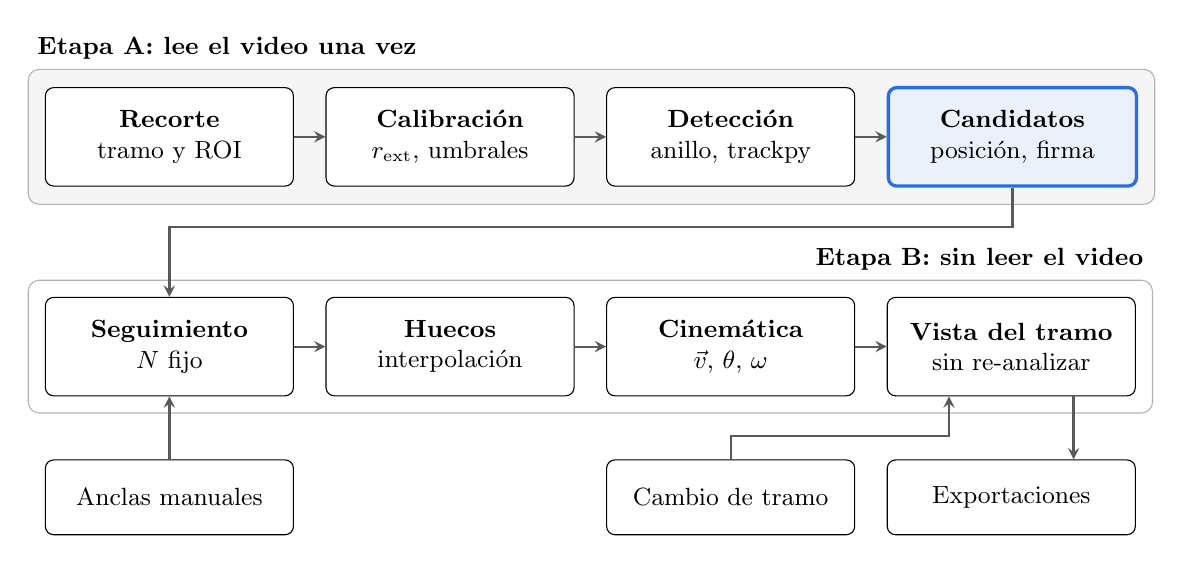
\begin{tikzpicture}[
      font=\small, node distance=4mm and 4mm,
      paso/.style={draw, rounded corners=3pt, align=center, minimum width=3.15cm, minimum height=1.25cm, fill=white},
      clave/.style={paso, draw=azul, very thick, fill=azul!10},
      ext/.style={paso, minimum height=0.95cm},
      flecha/.style={-stealth, thick, gray!70!black}]
    \node[paso]  (a1) {\textbf{Recorte}\\ tramo y ROI};
    \node[paso, right=of a1]  (a2) {\textbf{Calibración}\\ $r_{\mathrm{ext}}$, umbrales};
    \node[paso, right=of a2]  (a3) {\textbf{Detección}\\ anillo, trackpy};
    \node[clave, right=of a3] (a4) {\textbf{Candidatos}\\ posición, firma};
    \node[paso, below=14mm of a1] (b1) {\textbf{Seguimiento}\\ $N$ fijo};
    \node[paso, right=of b1]  (b2) {\textbf{Huecos}\\ interpolación};
    \node[paso, right=of b2]  (b3) {\textbf{Cinemática}\\ $\vec v$, $\theta$, $\omega$};
    \node[paso, right=of b3]  (b4) {\textbf{Vista del tramo}\\ sin re-analizar};
    \node[ext, below=8mm of b1] (c1) {Anclas manuales};
    \node[ext, below=8mm of b3] (c3) {Cambio de tramo};
    \node[ext, below=8mm of b4] (c4) {Exportaciones};
    \begin{scope}[on background layer]
      \node[draw=gray!60, fill=gray!8, rounded corners, inner sep=6pt, fit=(a1)(a4),
            label={[anchor=south west, font=\small\bfseries]north west:Etapa A: lee el video una vez}] {};
      \node[draw=gray!60, rounded corners, inner sep=6pt, fit=(b1)(b4),
            label={[anchor=south east, font=\small\bfseries]north east:Etapa B: sin leer el video}] {};
    \end{scope}
    \draw[flecha] (a1) -- (a2); \draw[flecha] (a2) -- (a3); \draw[flecha] (a3) -- (a4);
    \draw[flecha] (b1) -- (b2); \draw[flecha] (b2) -- (b3); \draw[flecha] (b3) -- (b4);
    \draw[flecha] (a4.south) -- ++(0,-5mm) -| (b1.north);
    \draw[flecha] (c1) -- (b1); \draw[flecha] (c3.north) -- ++(0,3mm) -| ($(b4.south west)!0.25!(b4.south east)$);
    \draw[flecha] ($(b4.south west)!0.75!(b4.south east)$) -- ($(c4.north west)!0.75!(c4.north east)$);
  \end{tikzpicture}
  \caption{Flujo de procesamiento.}
  \label{fig:flujo}
\end{figure}

\subsection{Sistema de referencia y unidades}

Las posiciones usan los ejes de la imagen: $x$ hacia la derecha, $y$ hacia abajo, con origen en la
esquina superior izquierda del recorte analizado. Los ángulos (dirección de la velocidad, $\theta$ y
$\omega$) son positivos en sentido antihorario visto en pantalla. La escala resulta de
\begin{equation}
  s = \frac{D}{2\,r_{\mathrm{ext}}}\quad\left[\si{\milli\metre\per px}\right],
\end{equation}
donde $r_{\mathrm{ext}}$ es el radio exterior del robot en píxeles medido por la calibración; su
incertidumbre (\SI{\pm 2}{\percent}) se propaga a todas las magnitudes en metros.

\paragraph{Video espejado.} Algunas cámaras graban la escena reflejada. Una reflexión invierte la
quiralidad: un giro horario se ve antihorario y viceversa. La opción \emph{Video espejado} de la
pestaña \emph{Seguimiento} corrige las exportaciones sin tocar el análisis, que siempre se hace sobre
la imagen tal como está (así la superposición coincide con el video). Para una reflexión respecto del
eje vertical de la imagen (\emph{horizontal}), con $W$ el ancho de la región analizada,
\begin{equation}
  x \to W - x,\qquad v_x \to -v_x,\qquad \theta \to -\theta,\qquad \omega \to -\omega ,
\end{equation}
y la dirección de la velocidad se recalcula; para una reflexión \emph{vertical} se cambian $y$ y $v_y$
en lugar de $x$ y $v_x$. El CSV lleva entonces la columna \texttt{espejo}, y las columnas
\texttt{x\_video\_px}, \texttt{y\_video\_px} quedan siempre en píxeles del archivo.

\begin{table}[H]
  \centering
  \caption{Magnitudes medidas.}
  \begin{tabular}{@{}llll@{}}
    \toprule
    Magnitud & Símbolo & Unidad & Definición \\
    \midrule
    Tiempo real & $t$ & \si{\second} & $t = n/\fr$, con $n$ el número de cuadro \\
    Posición & $x,\,y$ & \si{\metre} & centro del robot, ejes de imagen \\
    Velocidad & $v_x,\,v_y$ & \si{\metre\per\second} & $\mathrm{d}x/\mathrm{d}t$, $\mathrm{d}y/\mathrm{d}t$ \\
    Rapidez & $|\vec v|$ & \si{\metre\per\second} & $\sqrt{v_x^2+v_y^2}$ \\
    Dirección & $\varphi$ & \si{\degree} & $\operatorname{atan2}(-v_y,\,v_x)$; \SI{0}{\degree} = derecha \\
    Orientación & $\theta$ & \si{\degree} & giro acumulado desde el primer cuadro del tramo \\
    Velocidad angular & $\omega$ & \si{\degree\per\second}, \si{\radian\per\second} & $\mathrm{d}\theta/\mathrm{d}t$ \\
    \bottomrule
  \end{tabular}
\end{table}

\subsection{Calibración automática del tamaño}

Visto desde arriba, el robot es un disco claro (la pila) rodeado por un anillo oscuro (la placa).
Se usa una plantilla con un disco de radio $r_{\mathrm{int}} = 0{,}75\,r_{\mathrm{ext}}$ y un anillo
hasta $r_{\mathrm{ext}}$, y se barre $r_{\mathrm{ext}}$: la respuesta media de los $N$ picos más fuertes
es máxima cuando la plantilla coincide con el robot real (\cref{fig:calib}). A partir de
$r_{\mathrm{ext}}$ se derivan la escala de análisis ($24/r_{\mathrm{ext}}$, para trabajar siempre con
robots de unos \SI{24}{px} de radio), la separación mínima ($1{,}5\,r_{\mathrm{ext}}$) y el radio de
búsqueda del seguimiento ($0{,}625\,r_{\mathrm{ext}}$). Los umbrales de gris se fijan como fracción
del contraste medido entre anillo y disco, por lo que no dependen de la exposición.

\begin{figure}[H]
  \centering
  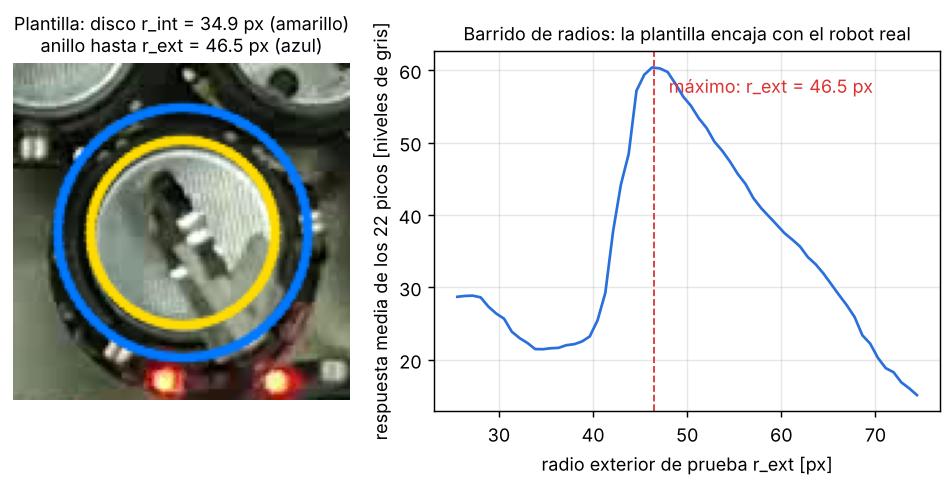
\includegraphics[width=0.9\linewidth]{figuras/metodo/f1_calibracion.png}
  \caption{Calibración: plantilla sobre un robot y respuesta en función del radio de prueba.}
  \label{fig:calib}
\end{figure}

\subsection{Detección}\label{sec:deteccion}

\paragraph{Filtro de anillo.} Para cada píxel se calculan el gris medio del disco y del anillo con
núcleos circulares normalizados, y se combinan como
\begin{equation}
  R(x,y) = \left(\mu_{\mathrm{disco}}-\mu_{\mathrm{anillo}}\right)\,
           \operatorname{clip}\!\left(\frac{G_{\max}-\mu_{\mathrm{anillo}}}{G_{\max}},\,0,\,1\right).
\end{equation}
El primer factor exige contraste; el segundo, que el anillo sea oscuro en valor absoluto. $R$ es alto
solo en los centros de los robots. En el código (\cref{lst:respuesta}), las medias locales son dos
convoluciones \texttt{cv2.filter2D} con núcleos normalizados a suma~1, calculadas sobre la imagen ya
reducida a la escala de análisis (los robots quedan con unos \SI{24}{px} de radio, lo que hace el
costo independiente de la resolución del video).

\begin{lstlisting}[caption={Filtro de anillo (\texttt{core/detection.py}).}, label=lst:respuesta]
def _disc_ring_kernels(r_in, r_out):
    R = int(np.ceil(r_out))
    yy, xx = np.mgrid[-R:R + 1, -R:R + 1]
    rr = np.hypot(xx, yy)
    disc = (rr <= r_in).astype(np.float32)
    ring = ((rr > r_in) & (rr <= r_out)).astype(np.float32)
    return disc / disc.sum(), ring / ring.sum()   # mean filters

def robot_response(gray, p):
    """Matched-filter map (uint8) at analysis scale."""
    ki, kr = _disc_ring_kernels(p.r_in * p.scale, p.r_out * p.scale)
    g = gray.astype(np.float32)
    m_disc = cv2.filter2D(g, -1, ki, borderType=cv2.BORDER_REFLECT)
    m_ring = cv2.filter2D(g, -1, kr, borderType=cv2.BORDER_REFLECT)
    gate = np.clip((p.ring_gray_max - m_ring) / p.ring_gray_max, 0.0, 1.0)
    return np.clip((m_disc - m_ring) * gate, 0, 255).astype(np.uint8)
\end{lstlisting}

\paragraph{Localización.} \texttt{trackpy.locate} busca los máximos locales de $R$ y devuelve su
centroide con precisión subpíxel. Se aplica sobre $R$ y no sobre la imagen porque la pila no es una
mancha uniforme: la palanca metálica y los reflejos corren el centroide. Los argumentos salen de la
calibración: el diámetro de la mancha buscada ($1{,}4\,r_{\mathrm{int}}$ en la escala de análisis,
redondeado a impar, porque el pico de $R$ es más angosto que el disco), la separación mínima entre
centros y \texttt{minmass}. Las coordenadas devueltas se dividen por la escala para volver a píxeles
del video (\cref{lst:locate}).

\begin{lstlisting}[caption={Llamada a trackpy (\texttt{core/detection.py}, función \texttt{locate}).}, label=lst:locate]
f = tp.locate(img, p.trackpy_diameter(), minmass=p.minmass,
              separation=max(1.0, p.separation * p.scale), invert=False)
f["x"] = f["x"] / p.scale          # back to video pixels
f["y"] = f["y"] / p.scale
\end{lstlisting}

\paragraph{Validación.} Un hueco de piso rodeado de robots también genera un pico, pero su ``anillo''
está formado por los vecinos y no es cerrado. Se trazan 360 rayos desde el centro y se exige que al
menos el \SI{82}{\percent} encuentre un píxel oscuro dentro de la banda del anillo
(\cref{fig:deteccion,fig:cobertura}). \texttt{cv2.warpPolar} desenrolla la imagen alrededor del
candidato: cada fila es un rayo y cada columna un radio, de modo que la cobertura es una sola
operación vectorizada (\cref{lst:cobertura}).

\begin{lstlisting}[caption={Cobertura angular del anillo oscuro (\texttt{core/detection.py}).}, label=lst:cobertura]
def ring_coverage(gray, x, y, r0, r1, dark):
    """Fraction of 360 rays whose darkest pixel in the band [r0, r1) is below `dark`."""
    r1i, r0i = int(np.ceil(r1)), int(max(0, np.floor(r0)))
    pol = cv2.warpPolar(gray, (r1i + 1, 360), (float(x), float(y)), r1i + 1,
                        cv2.WARP_POLAR_LINEAR)          # rows = angle, cols = radius
    return float((pol[:, r0i:r1i].min(axis=1) < dark).mean())
\end{lstlisting}

\begin{figure}[H]
  \centering
  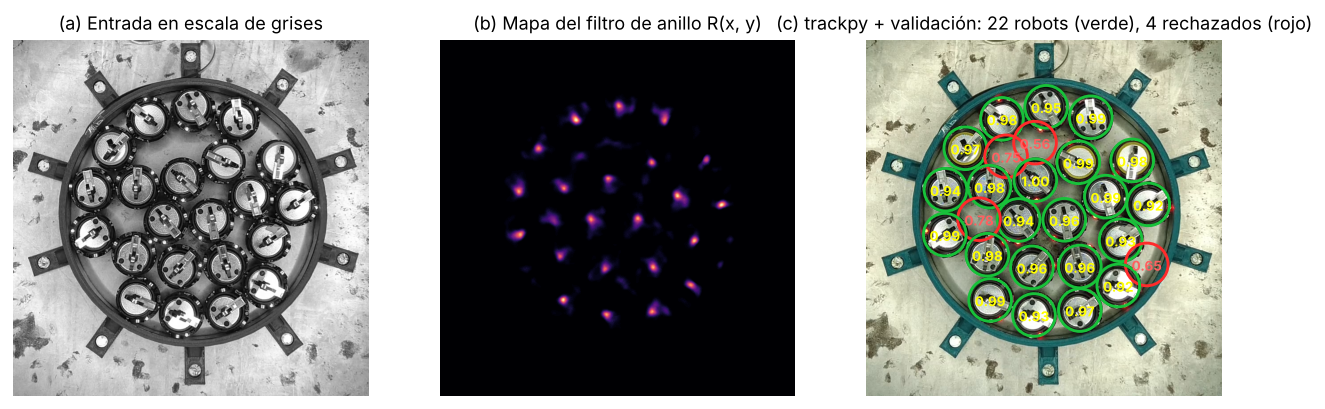
\includegraphics[width=\linewidth]{figuras/metodo/f2_deteccion.png}
  \caption{(a) Entrada. (b) Mapa $R$. (c) Candidatos con su cobertura: aceptados (verde) y huecos rechazados (rojo).}
  \label{fig:deteccion}
\end{figure}

\begin{figure}[H]
  \centering
  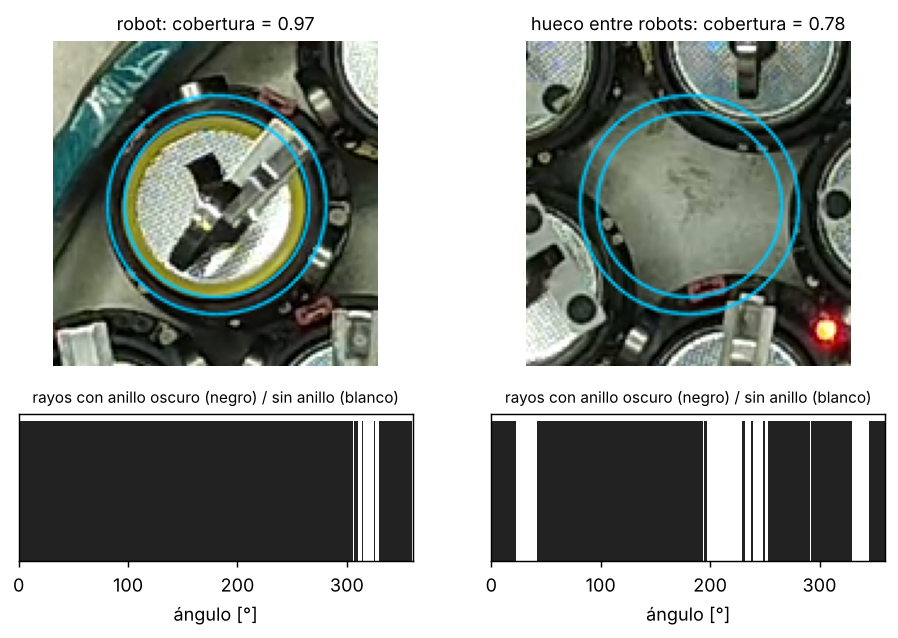
\includegraphics[width=0.72\linewidth]{figuras/metodo/f3_cobertura.png}
  \caption{Cobertura del anillo: un robot cierra el anillo en casi todos los rayos; un hueco, no.}
  \label{fig:cobertura}
\end{figure}

\subsection{Seguimiento con $N$ fijo}\label{sec:seguimiento}

En cada cuadro se predice la posición de cada robot (última posición más velocidad media reciente) y
se asignan predicciones y candidatos minimizando la distancia total (algoritmo húngaro), solo dentro
del radio de búsqueda. A los robots sin pareja se les ofrecen candidatos con umbrales relajados
(cobertura $\geq 0{,}70$ y luego $\geq 0{,}55$), pero solo cerca de su predicción. Un robot nuevo solo
se acepta si persiste en el \SI{75}{\percent} de los \Cuadros{20} siguientes. Los huecos acotados se
interpolan linealmente y cada punto queda con un estado (\cref{tab:estados}). Un centro marcado a mano
(ancla) es una restricción fija desde la que el seguimiento continúa (\cref{fig:seguimiento}).

El seguimiento corre en dos etapas. La etapa~A recorre el video una sola vez y guarda, para cada
cuadro, todos los candidatos con un umbral permisivo (cobertura $\geq 0{,}45$) y su firma de
rotación. La etapa~B trabaja solo sobre esa tabla: parte del cuadro con mejor detección y avanza
hacia adelante y hacia atrás. Cada robot guarda su última posición y una velocidad suavizada
exponencialmente ($\alpha = 0{,}5$); la predicción extrapola esa velocidad, limitada a
\texttt{max\_gap} cuadros para no alejarse demasiado en un hueco. La asignación usa
\texttt{scipy.optimize.linear\_sum\_assignment} con costo igual a la distancia, y costo prohibitivo
fuera del radio de búsqueda, que crece con la cantidad de cuadros sin detección
(\cref{lst:asignacion}).

\begin{lstlisting}[caption={Predicción y asignación con compuerta (\texttt{core/tracking.py}, resumido).}, label=lst:asignacion]
def predict(self, frame, max_gap):
    dt = frame - self.f                                   # signed: also runs backwards
    eff = np.sign(dt) * np.minimum(np.abs(dt), max_gap)   # damp long extrapolations
    return self.xy + self.v * eff[:, None], np.abs(dt)

def _gated_assign(pred, gates, cand):
    d = np.linalg.norm(pred[:, None, :] - cand[None, :, :], axis=2)
    cost = np.where(d <= gates[:, None], d, _BIG)          # outside the gate = forbidden
    r, c = linear_sum_assignment(cost)                    # Hungarian algorithm
    return [(i, j) for i, j in zip(r, c) if cost[i, j] < _BIG]

# per frame: manual anchors first, then the strict and the relaxed coverage levels
for cov_thr, gate_factor, status in levels:   # (0.82, 1, DETECTED), (0.70, 0.6, RELAXED), ...
    ks = np.flatnonzero(st.has & ~done)
    js = np.flatnonzero(~used & (cov >= cov_thr))
    for a, b in _gated_assign(pred[ks], base_gate[ks] * gate_factor, xy[js]):
        ...   # store position, status and candidate index; update the velocity
\end{lstlisting}

\begin{table}[H]
  \centering
  \caption{Estados de cada posición (columna \texttt{status}).}
  \label{tab:estados}
  \begin{tabular}{@{}lp{9.2cm}@{}}
    \toprule
    Estado & Significado \\
    \midrule
    detectado & asignado con el umbral estricto \\
    detectado (umbral relajado) & asignado con cobertura 0,55--0,82 cerca de la predicción \\
    manual & centro marcado a mano \\
    interpolado & hueco de hasta \Cuadros{15} entre dos detecciones (advertencia) \\
    predicho (revisar) & hueco más largo o sin detección de un lado (error) \\
    perdido & sin ninguna posición \\
    \bottomrule
  \end{tabular}
\end{table}

\begin{figure}[H]
  \centering
  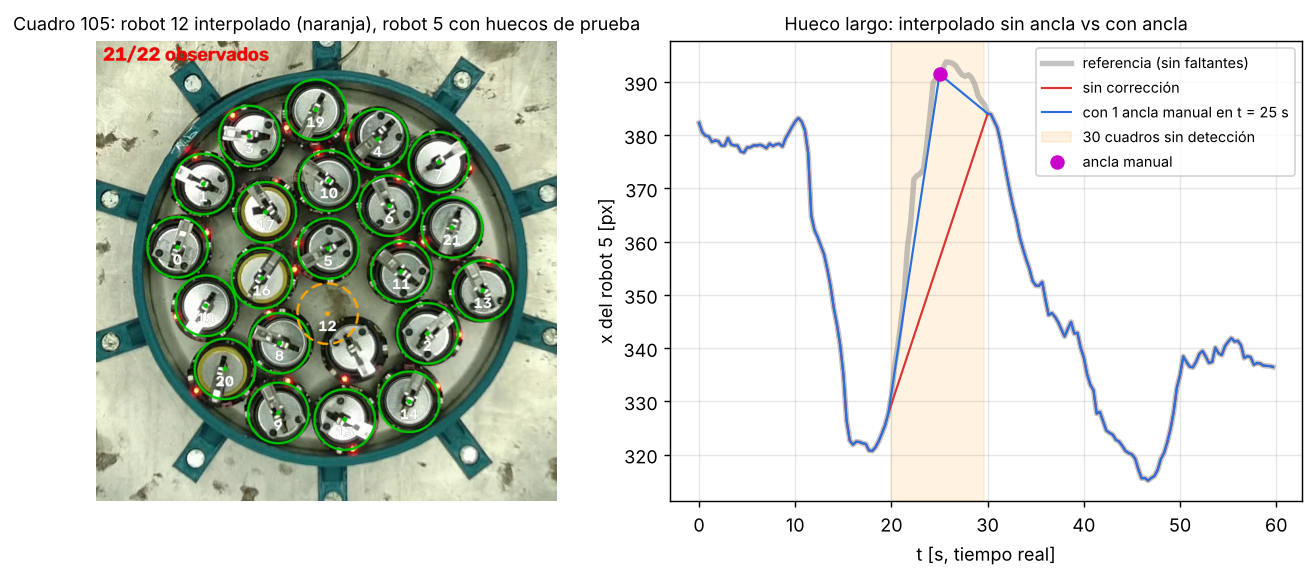
\includegraphics[width=\linewidth]{figuras/metodo/f4_seguimiento.png}
  \caption{Faltantes simulados: robot interpolado (naranja) y efecto de una sola ancla manual en un
    hueco de \Cuadros{30}. Tiempo real con $\fr = 3$~cuadros/s.}
  \label{fig:seguimiento}
\end{figure}

\subsection{Velocidad}\label{sec:velocidad}

El centro detectado fluctúa entre 1 y \SI{5}{px} por cuadro; una diferencia finita multiplicaría ese
ruido por $\fr$. Por eso la velocidad se obtiene con un filtro de Savitzky--Golay: para cada instante
se ajusta por mínimos cuadrados un polinomio de grado~2 a los cuadros vecinos (ventana de
\Cuadros{7} por defecto) y se toma su derivada analítica,
\begin{equation}
  v_x(t_i)=\left.\frac{\mathrm{d}\hat p_i}{\mathrm{d}t}\right|_{t_i},\qquad
  \hat p_i=\arg\min_{p\in\mathbb P_2}\sum_{j=-3}^{3}\bigl[x(t_{i+j})-p(t_{i+j})\bigr]^2 ,
\end{equation}
con $t_{i+j} = (i+j)/\fr$, y lo mismo para $v_y$ (\cref{fig:velocidad}). Una ventana mayor reduce
el ruido pero atenúa los cambios bruscos, como los choques. La ventana $w$ es un número de cuadros
(campo \emph{Suavizado} de la pestaña \emph{Seguimiento}): su duración real es $w/\fr$ y crece si
la captura es más lenta. En el código, \texttt{scipy.signal.savgol\_filter} con \texttt{deriv=1} y
\texttt{delta}$\,=1/\fr$ devuelve directamente la derivada por segundo real; los huecos
(\texttt{NaN}) se rellenan por interpolación solo para filtrar y se vuelven a marcar después
(\cref{lst:derivada}). La escala espacial se aplica al final:
$v\,[\si{\metre\per\second}] = v\,[\si{px\per\second}]\cdot s$.

\begin{lstlisting}[caption={Derivada temporal suavizada (\texttt{core/kinematics.py}).}, label=lst:derivada]
def _derivative(v, fps, p):
    """d/dt along axis 0 for each column; NaNs are bridged by interpolation, then restored."""
    out = np.full_like(v, np.nan, dtype=float)
    n = len(v)
    for k in range(v.shape[1]):                       # one column per robot
        col = v[:, k]
        ok = np.isfinite(col)
        if ok.sum() < 2:
            continue
        idx = np.arange(n)
        filled = np.interp(idx, idx[ok], col[ok])
        w = _odd_window(p.window, n, p.polyorder)
        d = savgol_filter(filled, w, p.polyorder, deriv=1, delta=1.0 / fps, mode="interp")
        d[~ok] = np.nan
        out[:, k] = d
    return out
\end{lstlisting}

\begin{figure}[H]
  \centering
  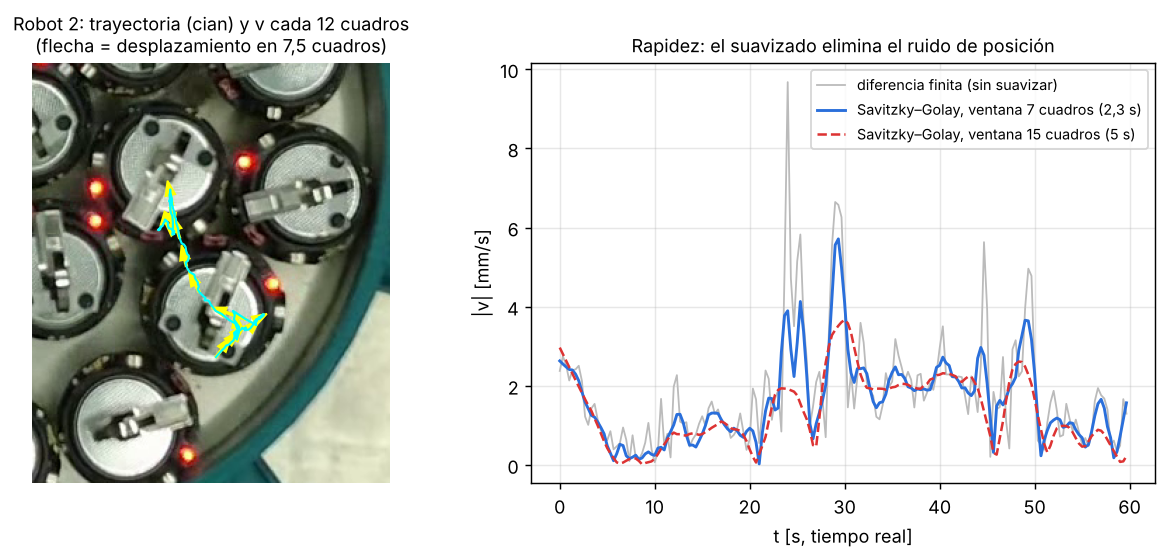
\includegraphics[width=\linewidth]{figuras/metodo/f5_velocidad.png}
  \caption{Trayectoria y vector velocidad de un robot (la flecha mide el desplazamiento en
    \num{7.5}~cuadros, por lo que su largo no depende de $\fr$); rapidez en tiempo real sin suavizar
    y con Savitzky--Golay, con $\fr = 3$~cuadros/s.}
  \label{fig:velocidad}
\end{figure}

\subsection{Orientación y velocidad angular}\label{sec:rotacion}

\paragraph{Firma de rotación.} Alrededor de cada centro la imagen se desenrolla en coordenadas
polares; una rotación del robot es entonces un corrimiento a lo largo del eje angular. En dos bandas
(pila, $0{,}15$--$0{,}70\,r_{\mathrm{ext}}$, y anillo, $0{,}75$--$0{,}95\,r_{\mathrm{ext}}$) se guarda el
perfil angular normalizado como sus primeros $K=12$ armónicos de Fourier (\cref{lst:firma}). Restar
la media de cada radio antes de promediar la banda elimina el gradiente radial de iluminación, y
normalizar por el desvío hace a la firma insensible al brillo de la escena.

\begin{lstlisting}[caption={Firma de rotación de un robot (\texttt{core/rotation.py}, resumido).}, label=lst:firma]
pol = cv2.warpPolar(gray, (R, 128), (x, y), R, cv2.WARP_POLAR_LINEAR)  # 128 angles x R radii
for b, (r0, r1) in enumerate(((0.15, 0.70), (0.75, 0.95))):            # battery, PCB ring
    band = pol[:, int(r0 * R):int(r1 * R)]
    prof = (band - band.mean(axis=0, keepdims=True)).mean(axis=1)      # angular profile
    prof = (prof - prof.mean()) / prof.std()
    sig[b] = np.fft.fft(prof)[1:13] / 128                              # harmonics 1..12
\end{lstlisting}

\paragraph{Ángulo entre dos cuadros.} El giro relativo es el máximo de la correlación circular de las
firmas,
\begin{equation}
  c(\Delta)=\operatorname{Re}\sum_b\sum_{k=1}^{K} S_2[b,k]\,\overline{S_1[b,k]}\,e^{ik\Delta},\qquad
  \Delta\theta=\arg\max_\Delta c(\Delta),
\end{equation}
refinado con dos pasos de Newton (error mediano \SI{0.37}{\degree} con rotaciones conocidas). Como
$c(\Delta)$ solo tiene armónicos hasta $K$, una grilla de 128 puntos (por FFT inversa) ubica el
máximo y la derivada analítica lo refina (\cref{lst:angulo}).

\begin{lstlisting}[caption={Giro relativo entre dos firmas (\texttt{core/rotation.py}, resumido).}, label=lst:angulo]
C = (s2 * np.conj(s1)).sum(axis=-2)                 # cross-spectrum, summed over bands
spec[..., 1:K + 1] = C
c = np.real(np.fft.ifft(spec, axis=-1)) * 128        # c(Delta) on a 128-point grid
d = np.argmax(c, axis=-1) * (2 * np.pi / 128)
k = np.arange(1, K + 1)
for _ in range(2):                                   # Newton on dc/dDelta = 0
    e = C * np.exp(1j * k * d[..., None])
    d1 = np.real((1j * k * e).sum(-1))
    d2 = np.real((-(k ** 2) * e).sum(-1))
    d = d - np.where(d2 < 0, d1 / d2, 0.0)
angle = -((np.degrees(d) + 180) % 360 - 180)         # CCW on screen (warpPolar is clockwise)
\end{lstlisting}

\paragraph{Ángulo acumulado.} Sumar solo giros entre cuadros consecutivos acumula el error de cada
paso. Cada cuadro se compara con los que están 1, 2, 4, 8 y 16 cuadros atrás y todos los ángulos se
resuelven juntos por mínimos cuadrados ponderados por la similitud $q$:
\begin{equation}
  \min_{\theta}\sum_{(i,L)} q_{i,L}\left(\theta_{i+L}-\theta_i-m_{i,L}\right)^2,\qquad \theta_0=0,
\end{equation}
con un error acumulado $\leq \SI{2}{\degree}$ en \num{3000}~cuadros. El sistema es ralo y de banda
(cada ecuación vincula dos cuadros separados a lo sumo 16), por lo que se arma con
\texttt{scipy.sparse.coo\_matrix} y se resuelve con las ecuaciones normales y \texttt{spsolve}, en
tiempo proporcional a la cantidad de cuadros. Las comparaciones largas con similitud $q<0{,}8$ o
que discrepan más de \SI{30}{\degree} de la cadena incremental se descartan. Finalmente
$\omega=\mathrm{d}\theta/\mathrm{d}t = \fr\,\mathrm{d}\theta/\mathrm{d}n$ con el mismo
Savitzky--Golay (\cref{fig:rotacion}). La
\cref{fig:desrotacion} verifica la medición: al girar cada imagen por $-\theta$, los LEDs y los puntos
de la placa quedan fijos, por lo que $\theta$ describe la orientación del cuerpo del robot (la palanca
de la pila gira levemente respecto de él y no sirve como referencia).

\begin{figure}[H]
  \centering
  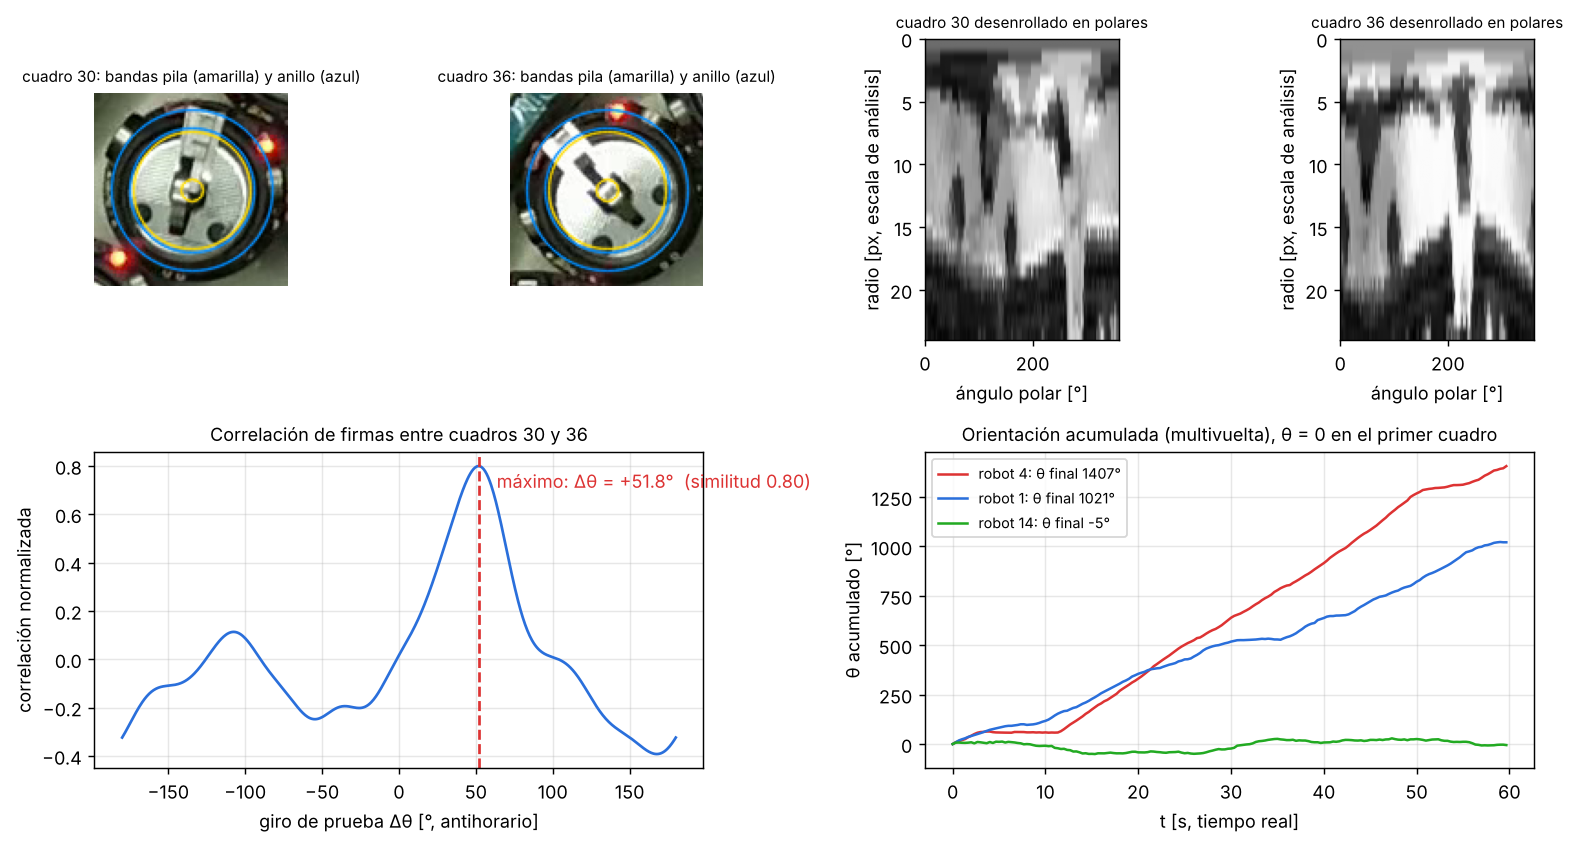
\includegraphics[width=\linewidth]{figuras/metodo/f6_rotacion.png}
  \caption{Firma polar en dos cuadros, correlación de las firmas y orientación acumulada de tres robots.}
  \label{fig:rotacion}
\end{figure}

\begin{figure}[H]
  \centering
  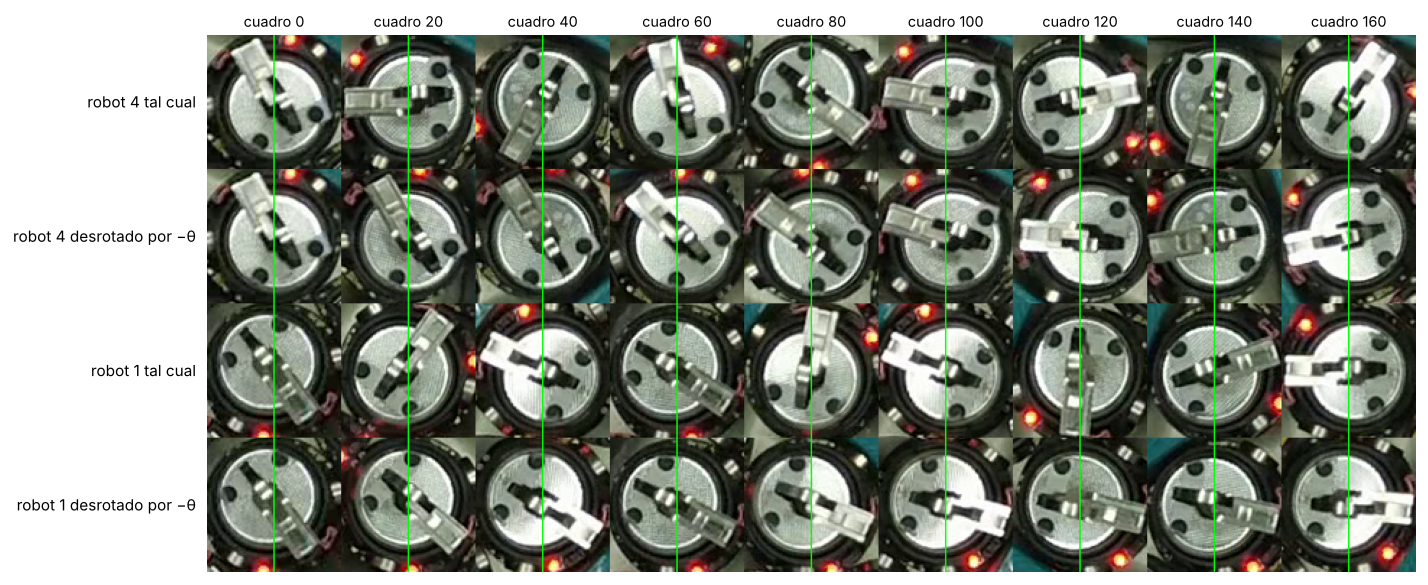
\includegraphics[width=\linewidth]{figuras/metodo/f7_desrotacion.png}
  \caption{Validación por desrotación: filas pares, las imágenes de la fila anterior giradas por $-\theta$.}
  \label{fig:desrotacion}
\end{figure}

\begin{figure}[H]
  \centering
  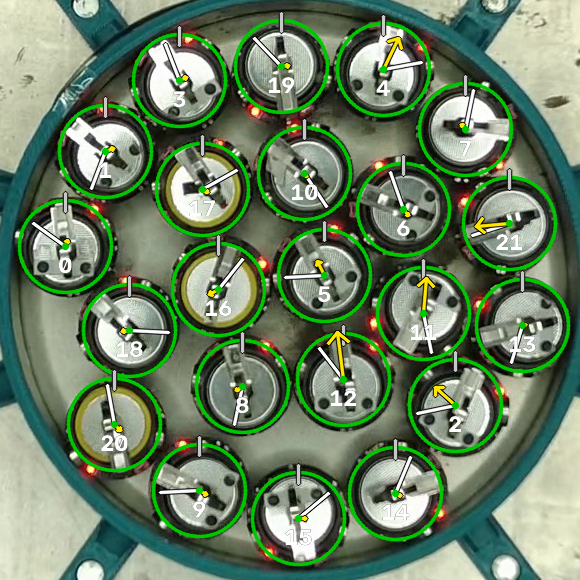
\includegraphics[width=0.6\linewidth]{figuras/metodo/f8_superposicion.png}
  \caption{Superposición en la aplicación: estado (color del círculo), velocidad (flecha amarilla,
    desplazamiento en \num{7.5}~cuadros) y orientación (aguja blanca; la marca a las 12~h es $\theta=0$).}
  \label{fig:superposicion}
\end{figure}

\subsection{Recorte temporal}

Si se recorta el tiempo después de analizar, los resultados se toman del análisis completo: las
derivadas conservan su precisión en los bordes y $\theta$ se re-referencia a cero en el primer cuadro
del tramo. Las exportaciones y este informe usan siempre el tramo vigente (\cref{sec:procedimiento}).

\subsection{Incertidumbres y limitaciones}

\begin{itemize}
  \item Posición: fluctuación de 1--\SI{5}{px} entre cuadros; escala espacial: \SI{\pm 2}{\percent}.
  \item Escala temporal: un error relativo en $\fr$ pasa sin atenuar a $|\vec v|$ y a $\omega$,
        según la \cref{eq:incert_t}; con $\fr$ estimado de la configuración de la cámara o del registro del
        sensor es del orden de \SI{1}{\percent}, con la duración nominal del nombre puede superar el
        \SI{10}{\percent}.
  \item Velocidad: los cambios más cortos que la ventana de suavizado (\EnSeg{7}) se atenúan, y nada
        más rápido que $\Delta t = \EnSeg{1}$ se resuelve.
  \item Orientación: \SI{\pm 0.4}{\degree} por comparación, $\leq \SI{2}{\degree}$ acumulado; en cuadros
        sin imagen del robot $\theta$ se interpola, y un giro mayor que media vuelta entre dos
        cuadros comparados no se detecta.
  \item Huecos: la interpolación lineal se aparta si el robot cambia de dirección; tras un hueco, un
        candidato aceptado con umbral relajado puede ser un falso positivo cercano a una predicción
        errónea. Para estadística conviene usar solo \texttt{status} = detectado.
\end{itemize}

% ============================================================================
% How to analyse a video and add it to this report; meaning of every export.
% ============================================================================
\section{Procedimiento y exportaciones}\label{sec:procedimiento}

\subsection{Analizar un video}

\begin{enumerate}
  \item \textbf{Abrir} el \texttt{VC\_<código>.MP4} (menú \emph{Archivo}, pestaña \emph{1 · Original}).
  \item \textbf{Escala de tiempo.} En la misma pestaña, dejar marcada \emph{Video acelerado
        (time-lapse)} y fijar $\fr$ (\cref{sec:escala}). Si se conoce la duración real medida,
        usar \emph{Calcular desde la duración real\ldots}.
  \item \textbf{Recorte} (opcional, pestaña \emph{2 · Recortar}): tramo temporal y rectángulo a analizar.
        Los \texttt{VC} ya están recortados a la arena, así que normalmente no hace falta.
  \item \textbf{Seguimiento} (pestaña \emph{4 · Seguimiento}): indicar $N$, verificar el diámetro real
        (\SI{35}{\milli\metre}), indicar si el video está espejado y pulsar \emph{Analizar video}. La calibración del tamaño es automática
        (casilla \emph{Calibrar tamaño automáticamente al analizar}).
  \item \textbf{Revisar} los cuadros de la lista \emph{Cuadros con problemas} (botones \emph{Anterior} y
        \emph{Siguiente}) y, si hace falta, elegir el robot y hacer clic sobre su centro real (ancla). El
        seguimiento se rehace en segundos, sin volver a leer el video.
  \item \textbf{Guardar} el análisis (\emph{Guardar análisis\ldots}, archivo \texttt{.npz}) y exportar el
        CSV con \emph{Exportar CSV (todos los robots)\ldots}, formato \emph{una fila por robot y cuadro}.
\end{enumerate}

\subsection{Generar el informe de ensayos}

Dos scripts de \nolinkurl{software/analisis_video/} arman el informe de resultados
(\nolinkurl{informes/ensayos/informe_ensayos.tex}) a partir de los CSV exportados. Se ejecutan desde
la raíz del repositorio; en Windows la línea se continúa con \verb|^| y en Linux o macOS con
\verb|\|. Por defecto escriben en \nolinkurl{informes/ensayos/generado/} y leen el registro de
presión de \nolinkurl{datos/presion/crudos/}.

\paragraph{Una sección por ensayo.} \texttt{generar\_informe.py} crea
\nolinkurl{generado/<nombre>/} con la tabla de datos, la captura anotada, los gráficos y un
párrafo automático, y actualiza \nolinkurl{generado/lista_ensayos.tex}:
\begin{verbatim}
python software/analisis_video/generar_informe.py ^
       datos/video/trayectorias/VP_20262409_1600_22QR_60_robots.csv ^
       --video datos/video/recortados/VC_20262409_1600_22QR_60.MP4 ^
       --nombre 20262409_1600_22QR_60
\end{verbatim}
Opciones:
\begin{itemize}
  \item \texttt{-{}-cuadros-por-segundo F}: reexpresa el CSV con $\fr = F$. Recalcula $t = n/F$ y
        multiplica velocidades y velocidades angulares por $F/\fr^{\mathrm{CSV}}$, donde
        $\fr^{\mathrm{CSV}}$ se deduce de las columnas \texttt{frame} y \texttt{t\_s}. Corrige un CSV
        exportado con otra escala sin repetir el análisis.
  \item \texttt{-{}-imagen archivo.png -{}-frame n}: usa una imagen ya extraída del cuadro $n$ para la
        captura anotada, en lugar de leer el video (útil si el video no está en la misma máquina).
  \item \texttt{-{}-titulo}, \texttt{-{}-diametro-mm}, \texttt{-{}-diametro-px} (si el CSV no trae escala).
\end{itemize}
Si la duración real supera \SI{10}{\minute}, los ejes de tiempo van en minutos y las trayectorias se
grafican solo para los primeros \SI{5}{\minute}. Las observaciones propias van en
\nolinkurl{generado/<nombre>/notas.tex}, que el script nunca sobrescribe. Si el CSV se exportó con
la corrección de video espejado (columna \texttt{espejo}), la captura se dibuja igual sobre la
imagen original.

\paragraph{Comparación entre ensayos.} \texttt{comparar\_ensayos.py} recibe todos los CSV y genera
\nolinkurl{generado/comparacion/}: tabla comparativa, series temporales con los atascos
marcados, distribuciones, rotación por robot, desplazamiento cuadrático medio, mapas de ocupación y,
si encuentra los registros del sensor, la alineación con el registro del sensor de presión
(\texttt{R\_<código>.csv}) mediante el pulso LED de sincronización y la correlación cruzada:
\begin{verbatim}
python software/analisis_video/comparar_ensayos.py ^
       "datos/video/trayectorias/VP_*_robots.csv"
\end{verbatim}
Después se compila \texttt{informes/ensayos/informe\_ensayos.tex} dos veces (\texttt{pdflatex} o
\texttt{latexmk -pdf}). Este informe (\texttt{informe\_aplicacion.tex}) no depende de los datos.

\subsection{Archivos exportados}

\paragraph{CSV de seguimiento (una fila por robot y cuadro).} Es el archivo de datos del ensayo y la
entrada del informe. Tiempos, velocidades y velocidades angulares están en tiempo real, con la
escala $\fr$ vigente al exportar (\cref{tab:columnas}).

\begin{table}[H]
  \centering
  \caption{Columnas del CSV de seguimiento.}
  \label{tab:columnas}
  \small
  \begin{tabular}{@{}llp{8.6cm}@{}}
    \toprule
    Columna & Unidad & Contenido \\
    \midrule
    \texttt{frame} & --- & número de cuadro $n$ en el archivo de video \\
    \texttt{t\_s} & \si{\second} & tiempo real $n/\fr$ \\
    \texttt{particle} & --- & identificador del robot ($0\ldots N-1$), fijo durante todo el ensayo \\
    \texttt{x\_px}, \texttt{y\_px} & px & centro, relativo al rectángulo analizado ($y$ hacia abajo) \\
    \texttt{status} & --- & estado de la posición (\cref{tab:estados}); \texttt{status\_code}, su código numérico \\
    \texttt{vx\_px\_s}, \texttt{vy\_px\_s} & \si{px\per\second} & componentes de la velocidad \\
    \texttt{speed\_px\_s} & \si{px\per\second} & rapidez $|\vec v|$ \\
    \texttt{vel\_dir\_deg} & \si{\degree} & dirección $\varphi$ de $\vec v$, antihoraria, \SI{0}{\degree} = derecha \\
    \texttt{theta\_deg} & \si{\degree} & orientación acumulada $\theta$, cero en el primer cuadro del tramo \\
    \texttt{omega\_deg\_s}, \texttt{omega\_rad\_s} & \si{\degree\per\second}, \si{\radian\per\second} & velocidad angular $\omega$ \\
    \texttt{rot\_status} & --- & \emph{medida}, \emph{interpolada} o \emph{no disponible} \\
    \texttt{x\_m}, \texttt{y\_m} & \si{\metre} & posición en SI (si se cargó el diámetro real) \\
    \texttt{vx\_m\_s}, \texttt{vy\_m\_s}, \texttt{speed\_m\_s} & \si{\metre\per\second} & velocidad en SI \\
    \texttt{mass}, \texttt{ring\_cov} & --- & intensidad de la detección y cobertura del anillo \\
    \texttt{x\_video\_px}, \texttt{y\_video\_px} & px & centro en coordenadas del video completo (sin corregir espejado) \\
    \texttt{espejo} & --- & solo si se corrigió el espejado: \texttt{horizontal} o \texttt{vertical} \\
    \bottomrule
  \end{tabular}
\end{table}

\paragraph{CSV de seguimiento (una fila por cuadro).} Mismos datos en formato ancho: una fila por
cuadro y, por cada robot $k$, las columnas anteriores con el prefijo \texttt{r}$k$\texttt{\_}
(\texttt{r00\_x\_px}, \texttt{r00\_y\_px}, \ldots). Cómodo para planillas; el informe usa el formato largo.

\paragraph{Resumen por robot.} Una fila por robot: duración (s reales), porcentaje de posiciones
observadas y de rotación medida, rapidez media y máxima, recorrido total, desplazamiento neto, giro
total y $\omega$ media y media en valor absoluto, en píxeles y en SI.

\paragraph{Video con seguimiento.} El tramo analizado con la superposición de la aplicación
(\cref{fig:superposicion}): círculo coloreado por estado, número de robot, flecha de velocidad
(desplazamiento en \num{7.5}~cuadros) y aguja de orientación. Se reproduce a $\fa$, igual que el original.

\paragraph{Sesión de análisis (\texttt{.npz}).} Guarda candidatos, firmas de rotación, anclas
manuales y resultado del seguimiento, para retomar el trabajo sin volver a leer el video. Al
cargarla se aplica la escala de tiempo vigente en la aplicación.


\end{document}
